This chapter presents the implementation of a custom software tool, which creates panoramic images based on point clouds captured, for example, via laser scanning. We discuss every step in the development phase from concept to finished prototype. It is developed with the version control system git and hosted in a public repository on GitHub.com. The software development progress is recorded via screen capturing and will gradually be uploaded online. Additionally, this information is provided on the official website which accompanies our research.

\section{Concept and preparation}

Based on the initial idea to somehow move from a dense point cloud to a 3D mesh surface that can be used in the 3D graphic suite Blender, it was important to plan ahead.\\
It is possible to mesh a 3D point cloud with several algorithms by, for example, trying to find the nearest neighbour of a point in 3D space. One such algorithm is called Delaunay Tetrahedralization  (see Shewchuk 2002 \parencite{Shewchuk02constraineddelaunay}) and is used in the free multi-view reconstruction software "Visual SFM" (see Appendix \ref{appendix_visual_sfm}), for instance.\\
With our method we try to utilize the characteristics of laser scanners in such a way that we know every aquired point can be described by scaling and rotating a unit sphere. In mathematical terms we can determine the spherical coordinates of every point in our point cloud. The 3D points need to be converted from their cartesian coordinate system to the spherical coordinate system first (see Wikipedia 2015 \parencite{wiki:CoordinateSystem}). Using this simple principle we can not only mesh a point cloud generated by a laser scanner, we can texture it, too. With the coordinates ranging from 0 to 360 degrees horizontally, 0 to 180 degrees vertically and a depth coordinate ranging from 0 to the maximum scan distance we are able to create two images, namely a depth map and a color map. Those images are then used to create a regular grid which is used for meshing and texture coordinates. By applying the inverse transform to the spherical coordinates it is possible to get the vertices of the textured 3D mesh in cartesian space and export it to any 3D file format. This process is explained in more detail in this chapter.\\
Furthermore it was neccessary to know how the user will be operating with the software. Usually a use case diagram is created to determine the required functions the software must provide in order to let a user accomplish his or her desired goals.

\subsection{Use case diagram}

The use of the converter software should be easy and fast. A user needs to do at least two actions, namely load a point cloud file and easily start the conversion process. Users should be able to adjust various settings for the file import, to meet the needs for their specific project. The initial use case diagram for this software looks like this:

\begin{figure}[h]
	\centering
	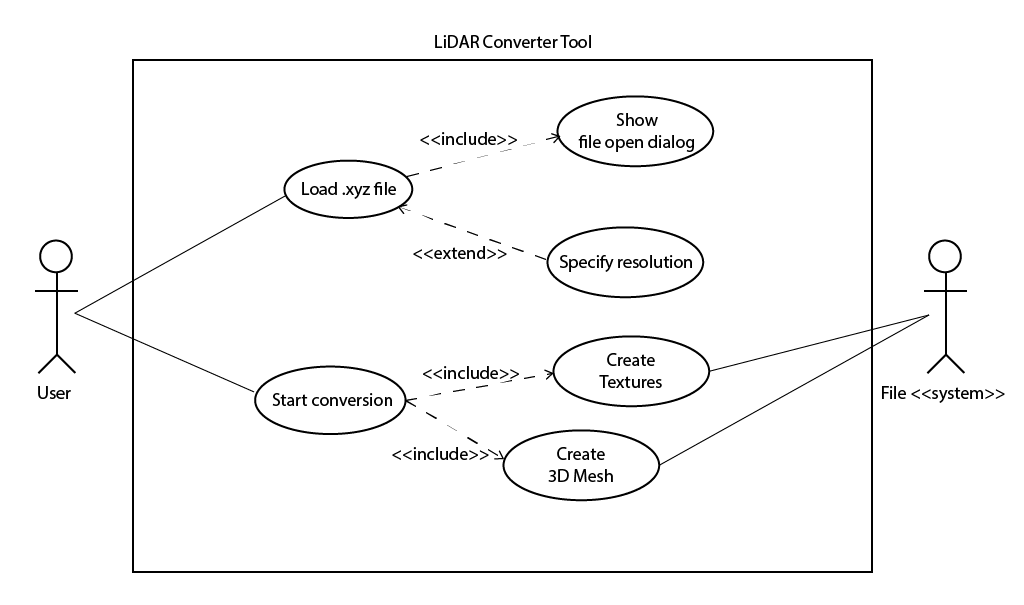
\includegraphics[scale=0.4]{UseCaseDiagram_PC2B.png}
	\caption{Use Case Diagram}
	\label{fig:use_case}
\end{figure}


\subsection{Laser scanning on location}

For data aquisition we used the FARO Focus\textsuperscript{3D} laser scanner on January 21st 2015. First, the device should be configured by setting the desired resolution (both for scan and photos), maximum scan distance (which results in a change of the eye-safety distance), a project name and GPS location (if no GPS module is available, as in our case). This configuration can be done in the office or on-site. After the device is set up, the scan process is started. During scanning, the main body of the device rotates horizontally and a mirror mounted inside the body rotates vertically. This creates the uncolored point cloud. After the scanning process, several pictures are taken by the built-in camera to color the point cloud. The scanner also measures the exposure to avoid under- or overexposured photographs. Finally, the inclination is measured with an inclinometer to level the point cloud properly. Scanning took about 40 minutes.
This procedure was repeated five times to get additional scans covering viewpoints that have been obstructed by obstacles.

During scanning we faced problems we didn't expect. We encountered people walking or stopping in the laser beam (resulting in vertical lines in the final scan), a suprising crash of the device's operating system leading to a terminal output window (wrecking the sd card with all previous scans), and a man asking if we took a photo of him while he was entering the building (obviously blocking the scanner while talking to us).

\begin{figure}[h]
	\centering
	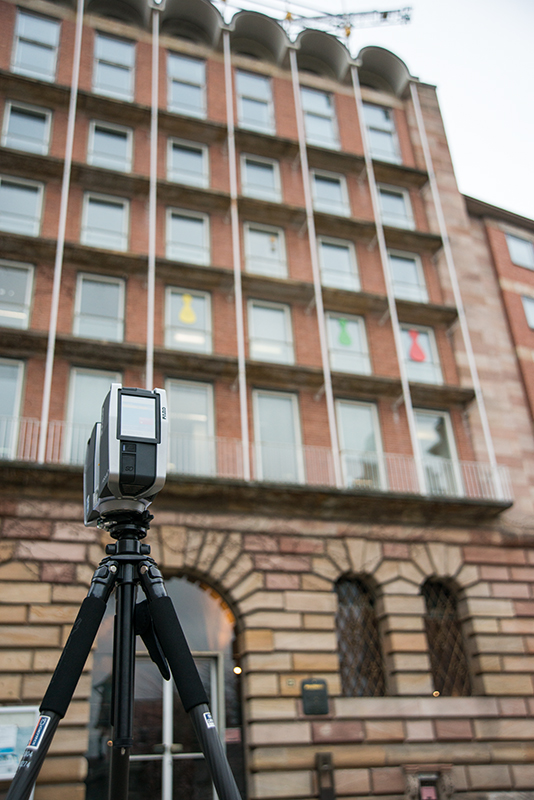
\includegraphics[scale=0.4]{PellerhausLaserScan.jpg}
	\caption{Scanning with FARO Focus\textsuperscript{3D}}
	\label{fig:laser_scanning_on_location}
\end{figure}


\section{Generating data and testing algorithms}

\subsection{BlenSor}

The Blender Sensor Simulation Toolbox (see Gschwandtner et al. 2011 \parencite{Gschwandtner11b}) is a custom version of the open source software Blender that allows simulations of different ways of scanning within a virtual 3D scene. It is being developed by the Department of Computer Sciences, University of Salzburg, Austria. The goal of this project is to provide a tool, mostly aimed at researchers, that can help with testing algorithms for fields such as obstacle detection and tracking, range data segmentation or surface reconstruction.\\
We found this software very useful to begin the development of PC2B. With a number of scanner presets it is possible to generate a point cloud of a virtual environment from different types of scanner devices.

\subsection{Test-Add-on for Blender}

During the beginning of the software development process the point cloud projection did not seem to be correct. Testing the algorithm responsible for projecting from cartesian to spherical coordinates was very tedious, because it involved importing the files, waiting for the images to get generated and then either looking at the produced image files to find mistakes or continuing with the meshing process. This pipeline was prone to errors, because one tiny mistake might affect the overall result.\\
Hence, a custom add-on for Blender was developed to test the equirectangular projection algorithm for correct mathematics. The language used for add-ons is Python 3 and enables developing powerful extensions to the Blender core.

\begin{figure}[h]
	\centering
	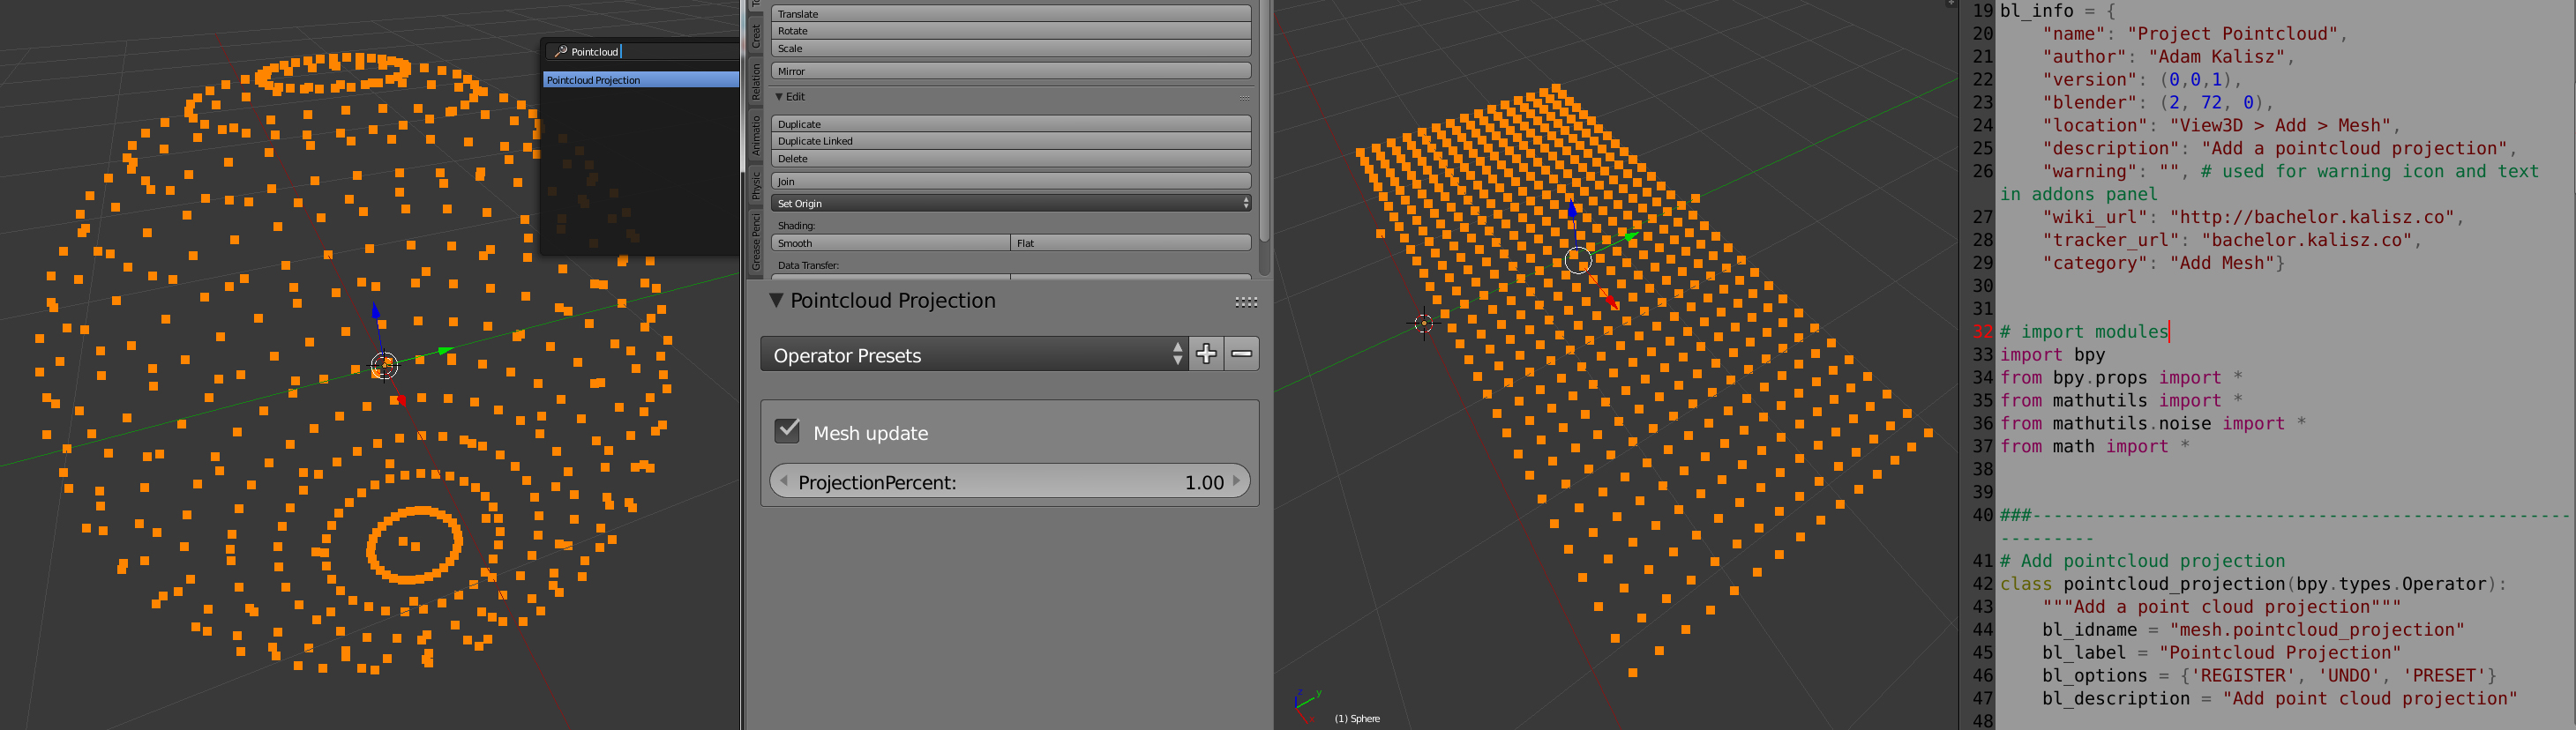
\includegraphics[width=1\textwidth]{BlenderAddon.jpg}
	\caption{Custom Blender Addon}
	\label{fig:blender_addon}
\end{figure}

A more efficient and elegant approach would be to develop a new modifier in C/C++ that integrates directly into Blender and can perform mesh manipulation fast. Unfortunately diving into Blender Core Development is not very easy due to its huge code base. In addition the time constraint did not permit experimenting further with this approach. Overall, it was helpful for tweaking the algorithm.

\section{Prototype}

The working title of this converter software was defined as "PointCloud2Blender", PC2B in short, because converting point clouds to a Blender compatible file format was the main goal of the software project. The prototype consists of three main parts: the importer, the 3D panorama, and the mesher. Additionally, an OpenGL viewer is implemented to visualize the data while it is being processed. A programming language and framework that provide the necessary performance and graphical user interface were needed. We decided to use C++ with Qt 5 for this task.

\subsection{UML class diagram}

PC2B was developed using object-oriented programming (OOP). To encapsulate certain properties and actions by creating and using objects, those are represented as classes in the source code. PC2B consists of several classes.\\
Helper classes, such as \textit{Point3D} and \textit{FileType}, provide clear representations of entities while still being flexible for future extensions. Graphical User Interface (GUI) code is contained in \textit{MainWindow}, which inherits from \textit{QMainWindow}. This \textit{MainWindow} is made visible in an instance of a \textit{QApplication} when the program is launched and creates user interface elements as well as instances of PC2B's main components responsible for processing LiDAR data. One of those component parts is the \textit{ImportWorker} which inherits from \textit{QRunnable} and enables it to run on a separate thread in a \textit{QThreadPool}. This is important, because reading and parsing a 6 GB point cloud file can take several minutes which freezes the main GUI loop if on the same thread. The same applies to \textit{MeshWorker} which implements the meshing algorithm and exports the final textured mesh for use in 3D applications. The \textit{Panorama3D} class encapsulates methods to convert a 3D point to a 2D pixel and vice versa. Additionally, it stores the panorama images. Finally the OpenGL viewer is implemented in two classes, \textit{GLWidget} which inherits from \textit{QGLWidget}, and \textit{GLMesh}. While \textit{GLWidget} provides a canvas to draw 3D graphics onto it via OpenGL, \textit{GLMesh} represents the 3D point cloud mesh and groups every property such as vertices, colors and shaders.\\
This relationship between individual objects is usually depicted in the Unified Modeling Language (UML) as a class diagram. Below is an example how a simplified UML class diagram for PC2B would look like:

\begin{figure}[h]
	\centering
	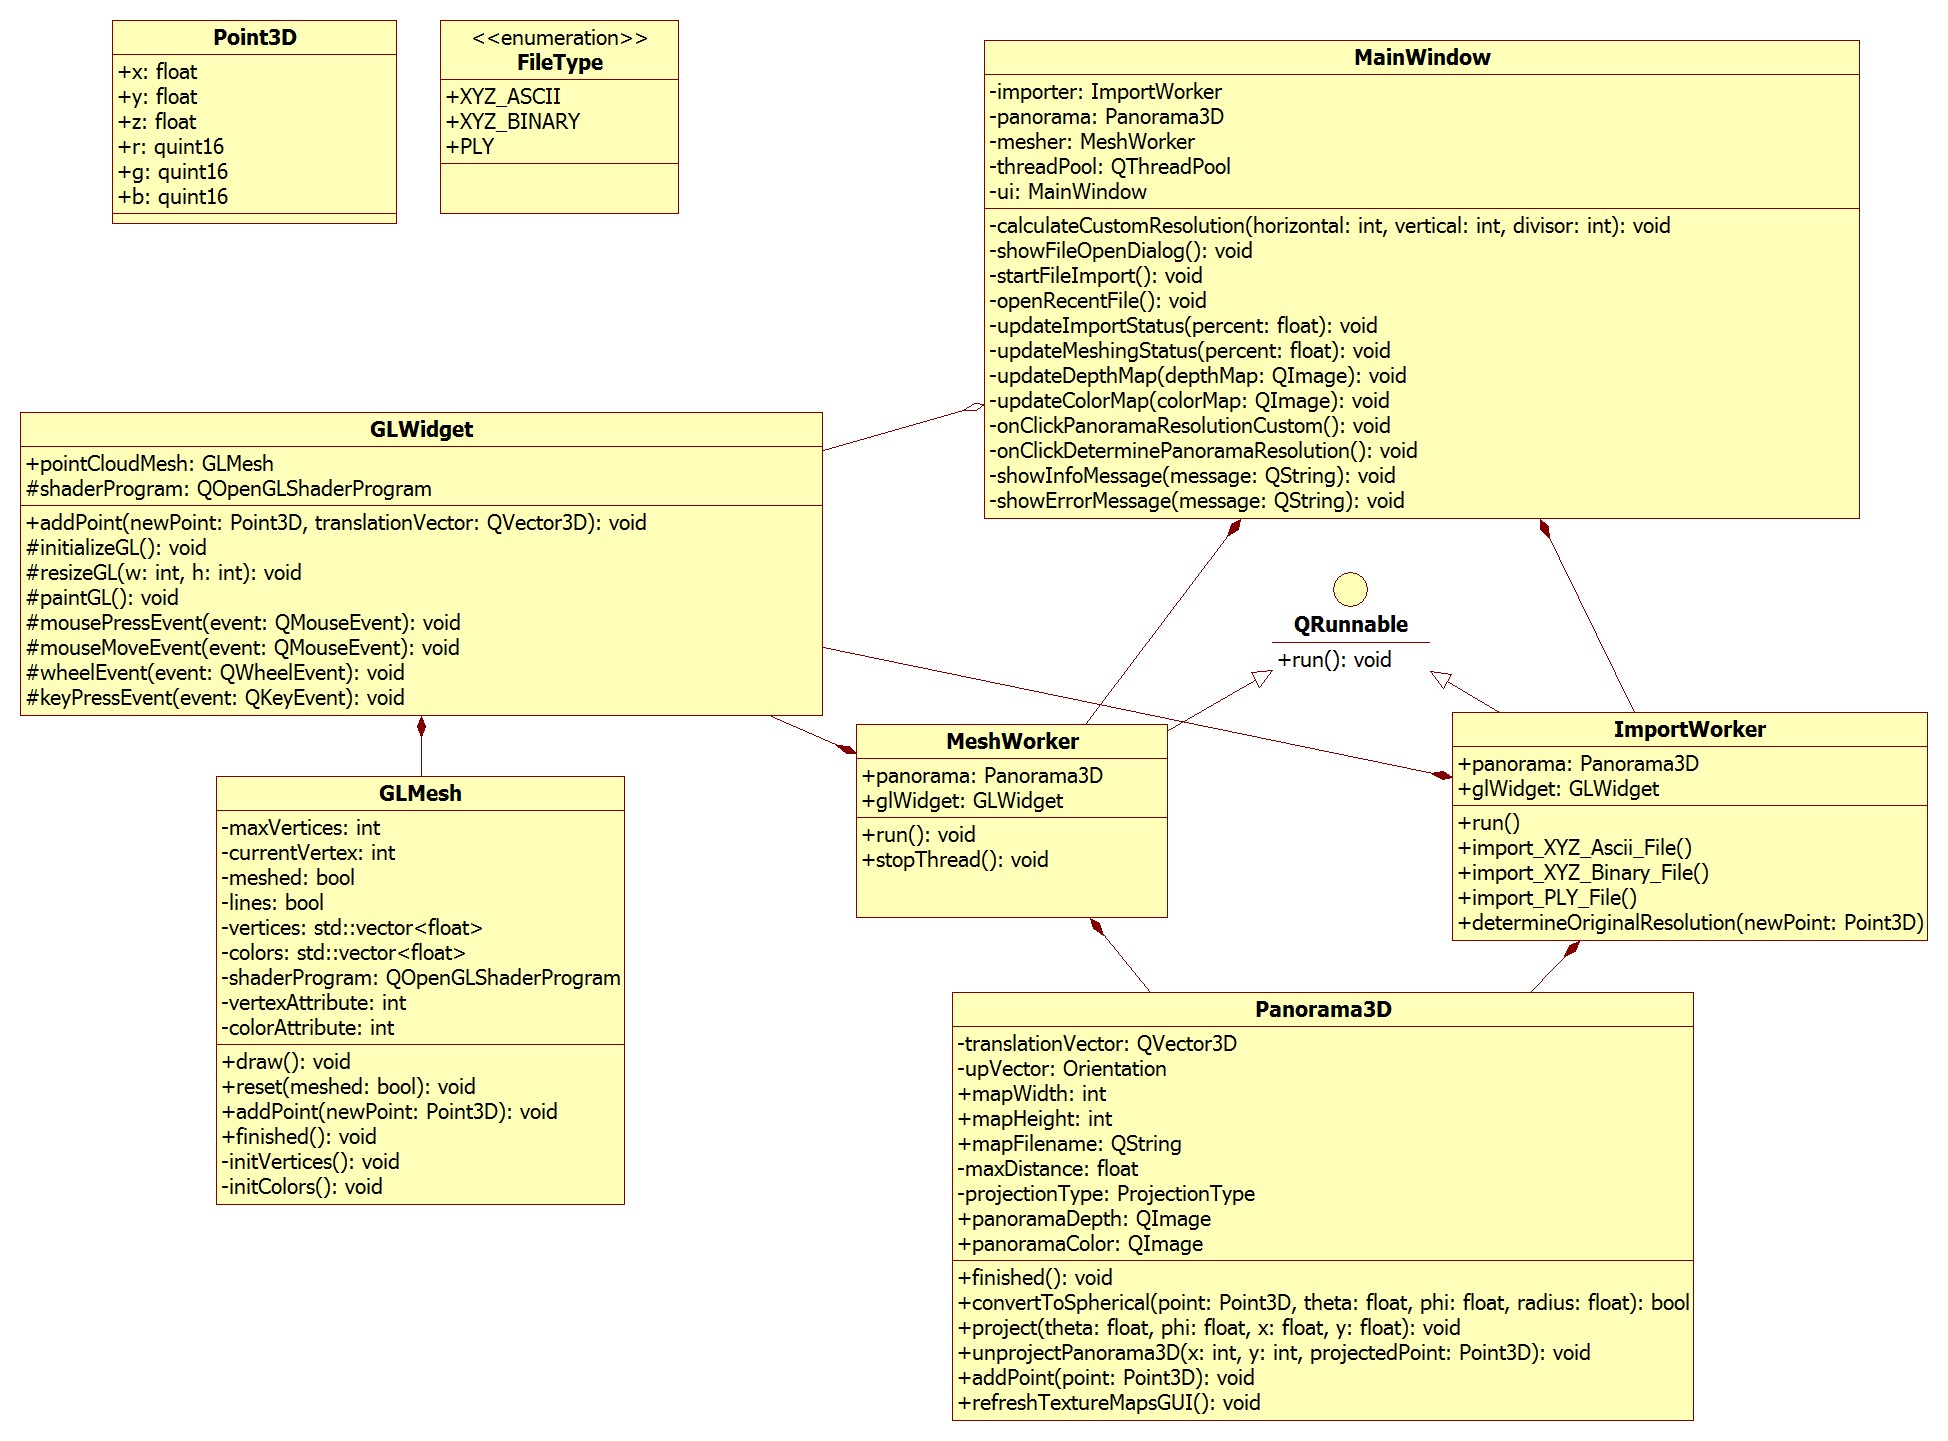
\includegraphics[width=1.0\textwidth]{PC2B_UML_class_diagram.jpg}
	\caption{PC2B UML class diagram (simplified)}
	\label{fig:pc2b_uml_class_diagram}
\end{figure}

\subsection{Point Cloud Importer}

A crucial part of the PC2B converter software is the ability to import point clouds saved as files. There is a huge amount of file types that can accomodate such a data structure. Points can be stored in ASCII, Binary or a hybrid form of both. ASCII files are human-readable, while binary are not. Importing binary formats requires one to know the exact structure of the file and the byte lengths used for certain values. This is important to avoid mixing and misinterpretation of data. A precise import function needs to adhere to the exact file structure rules. Documentation was limited for many of the file formats, so using ASCII files was a better choice from the beginning. Initially, it was decided to only import the .xyz file format, since this is a very simple file format that can be exported in ASCII form from the proprietary FARO SCENE 5 software which is needed for preprocessing the raw point cloud stream produced by the FARO Focus\textsuperscript{3D}.\\
During development it turned out that support for the .ply file format is desirable, since scientific websites that provide models (see Stanford Computer Graphics Laboratory 2014 \parencite{Stanford_repo}) widely provide this file type. Also Blender can export a 3D model to this file format. This fact was extremely useful for testing the algorithm, which is described later.

\subsubsection{Point Cloud data formats}

Working with such file structures, as in our case, is very easy (See Figure \ref{fig:xyz_ply_file_structure}).


\begin{figure}[h]
	\centering
	\begin{subtable}[b]{0.53\textwidth}
		
		\resizebox{\textwidth}{!}{%
		\begin{tabular}{l}
			-59.43620000 -31.36650000 302.80950000 59 46 55 \\
			-60.34600000 -31.80190000 302.85280000 58 45 54 \\
			-60.51810000 -31.88870000 302.71900000 58 45 54 \\
			-59.50470000 -31.39880000 302.68240000 56 47 50 \\
			-60.32350000 -31.79130000 302.89580000 59 46 54 \\
			-59.40940000 -31.35360000 302.85200000 61 48 57 \\
			-67.58220000 -29.73320000 302.12780000 73 55 58 \\
			-67.51000000 -29.59980000 302.04520000 63 43 54 \\
			-66.18880000 -29.78650000 299.88830000 100 87 80 \\
			-67.54620000 -29.66590000 302.08650000 64 47 56 \\
			-67.50660000 -29.59690000 302.00010000 62 43 51 \\
			-67.51970000 -29.60540000 302.09000000 64 46 57 \\
			...
		\end{tabular}}
		\caption{Sample .xyz file}
		\label{tab:xyz_file}
	\end{subtable}
	\hfill
	\begin{subtable}[b]{0.46\textwidth}
		\resizebox{\textwidth}{!}{%
		\begin{tabular}{l}
			ply \\
			format ascii 1.0 \\
			comment VCGLIB generated \\
			element vertex 2900882 \\
			property float x \\
			property float y \\
			property float z \\
			property uchar red \\
			property uchar green \\
			property uchar blue \\
			element face 1473375 \\
			property list uchar int vertex\_indices \\
			end\_header \\
			-37.037369 -0.850013 -1.831357 119 108 103 \\
			-37.063740 -0.755348 -1.886383 130 118 113 \\
			-37.446922 -0.902575 -2.421639 155 146 142 \\
			-37.512043 -1.051430 -2.535675 135 125 122 \\
			-37.546394 -0.904681 -2.498151 140 130 127 \\
			-37.340092 -0.932499 -2.274875 138 128 124 \\
			-37.292992 -0.973793 -2.336324 162 153 149 \\
			-37.166294 -0.780378 -2.111366 138 127 121 \\
			-37.341915 -0.864522 -2.316645 173 165 160 \\
			-36.981441 -0.691213 -1.978962 127 114 108 \\
			-36.918392 -0.767583 -1.994380 127 114 107 \\
			-37.038353 -0.931582 -2.136851 134 122 117 \\
			...
			
		\end{tabular}}
		\caption{Sample .ply file}
		\label{tab:ply_file}
	\end{subtable}
	\caption{Sample generated point cloud files}
	\label{fig:xyz_ply_file_structure}
\end{figure}

While the .xyz file type solely lists the x, y, z coordinates and optionally the red, green and blue color components, the .ply file type begins with a header describing how the file is structured. This has advantages, because we noticed that the .xyz file format is not documented. And to make things more complicated the free version of the proprietary FARO SCENE software, FARO SCENE LT, exports a different .xyz file than the paid version. With the free version two additional columns are added at the beginning of each row, such as the row and column number, and other settings can alter the file format even more. Those special cases are considered in the implementation of our prototype.


\subsection{Determination of original point cloud resolution}

Users of PC2B have the option to automatically determine the resolution of a 3D panorama based on the point cloud file. The 3D panorama resolution can either be set to fixed multiples of 360 by 180 pixels or set to a custom resolution, which can be filled out by the software. We have implemented an algorithm to help the user find the best resolution for his particular point cloud. It works by creating a histogram for counting the number of fixed steps of horizontal angles. First, we define an angle accuracy $\Delta{w}$:

$$ \Delta{w}=  \frac{\frac{360}{30000}}{4} $$

We limit the maximum horizontal scan points to 30,000 which returns an angle accuracy of 0.003 degrees. The histogram is created with $n$ values based on the accuracy:

$$ n = \left\lceil \frac{360}{ \Delta{w} } \right\rceil $$

For every scan point in the point cloud file, we compute its position (or index) in the histogram:

$$ i = \left\lfloor \frac{w}{ \Delta{w} } \right\rfloor $$

We then increment the histogram value at the index and repeat this procedure for every point in the point cloud file. The horizontal scan resolution is determined by counting the non-zero values in the histogram.


\subsection{Coordinate system representations}

We can express points in different coordinate systems, including cartesian, cylindrical and spherical.

Almost all point cloud files use a cartesian coordinate system (at least the ones we are using). To get the coordinate of a point in an image plane from a point in cartesian space, we simply convert its coordinate space from cartesian to spherical and project it onto the image plane. We then have the points horizontal position in a range of 360 degrees and its vertical position in a range of 180 degrees. In that way we create the image files from the point samples and then use those images to convert back to the cartesian space when creating the 3D mesh.

\subsection{Converting from cartesian to spherical and vice versa}

To convert from Cartesian space {$(x, y, z)$} to spherical coordinates {$(\theta, \varphi, radius)$}, we use the following equation:

$$radius = \sqrt{ (x^2 + y^2 + z^2) } $$
$$\theta = {\rm atan2} \left(y , x\right) + \pi$$
$$\phi = \cos^{-1} (z / radius)$$

Conversely, to get from spherical {$(\theta, \varphi, radius)$} to cartesian {$(x, y, z)$} coordinates (see Pharr et al. 2010 \parencite{Pharr:2010:PBR:1854996}, page 114), we use:

$$x = radius \cdot \sin \theta \cdot \cos \phi$$
$$y = radius \cdot \sin \theta \cdot \sin \phi$$
$$z = radius \cdot \cos \theta$$

\subsection{Types of projections}

To calculate the image pixels {$(x, y)$} from spherical coordinates, we have the option to use various projection types, as already briefly introduced in Section \ref{section_types_of_projections}. Their respective formulas are as follows (see Houshiar et al. 2015 \parencite{houshiar2015a}):

\subsubsection{Equirectangular projection}

$$I_x = \theta$$
$$I_y = \varphi$$

\subsubsection{Cylindrical projection}

$$I_x = \theta$$
$$I_y = \tan(\varphi) + \pi$$

\subsubsection{Mercator projection}

$$I_x = \theta$$
$$I_y = \ln \left(  \tan \left( \varphi \right) +  \left( \frac{1}{ \cos(\varphi) } \right) \right)$$

\subsection{Saving textures}

\begin{figure}[h]
	\centering
	\begin{subfigure}[b]{0.45\textwidth}
		\centering
		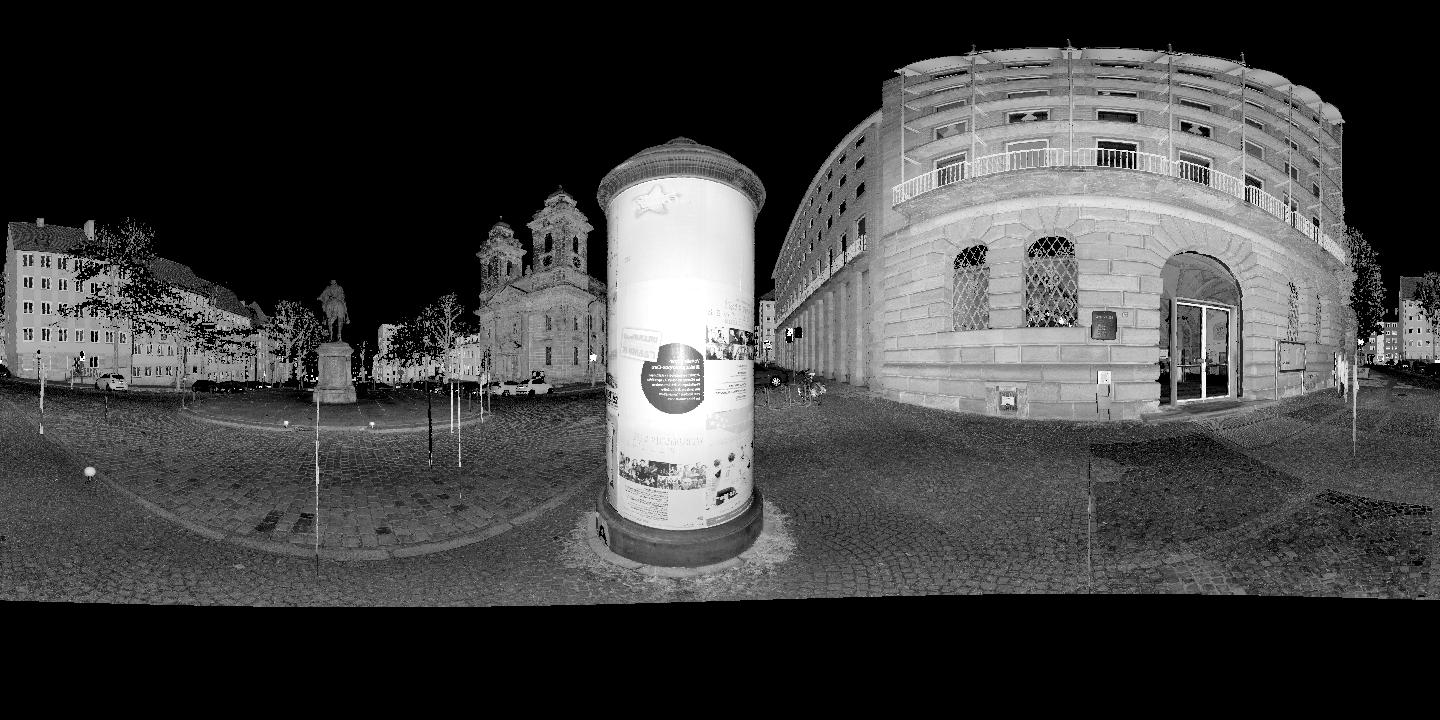
\includegraphics[width=\textwidth]{PC2B_colormap_grey.jpg}
		\caption{Colormap}
		\label{fig:PC2B_colormap_grey}
	\end{subfigure}
	\hfill
	\begin{subfigure}[b]{0.45\textwidth}
		\centering
		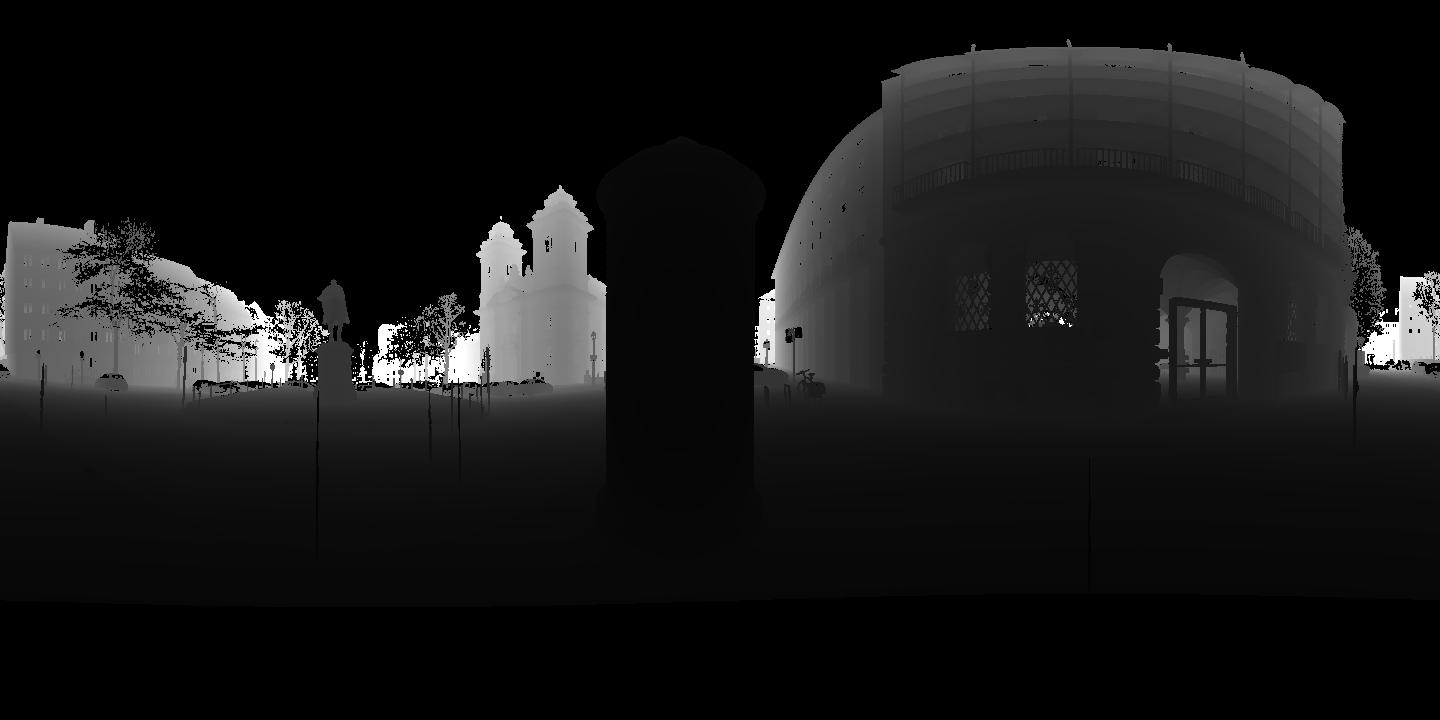
\includegraphics[width=\textwidth]{PC2B_depthmap.jpg}
		\caption{Depthmap}
		\label{fig:PC2B_depthmap}
	\end{subfigure}
	\caption{Panoramic images generated from the imported point cloud}
	\label{fig:PC2B_Panorama_images}
\end{figure}

At this point, each new row in the point cloud file returns the following data: x, y, z, r, g, b, radius, $\theta$, $\varphi$,  $I_x$ and  $I_y$. This enables us to create the panorama image files. The colormap image is formed from $I_x$, $I_y$, r, g and b. The depthmap is created from $I_x$, $I_y$ and radius. As the names imply, the colormap is necessary to color the 3D panorama (it will be applied as a texture for the 3D panorama) and the depthmap is used for displacing the individual vertices from the center by their depth value. The generated depth and color maps are stored with 8-bit unsigned integer values ranging from 0 to 255. After the point cloud file has been imported they are automatically saved as .jpg image files.

\subsection{Meshing}

After the panorama images have been created, the depthmap image is used for meshing. This is accomplished by looping through the individual pixels of the image and creating four-sided polygons (dashed line in red) clockwise from the current pixel (shaded green) and the neighboring pixels to the right, bottom-right and bottom.

\begin{figure}[h]
	\centering
	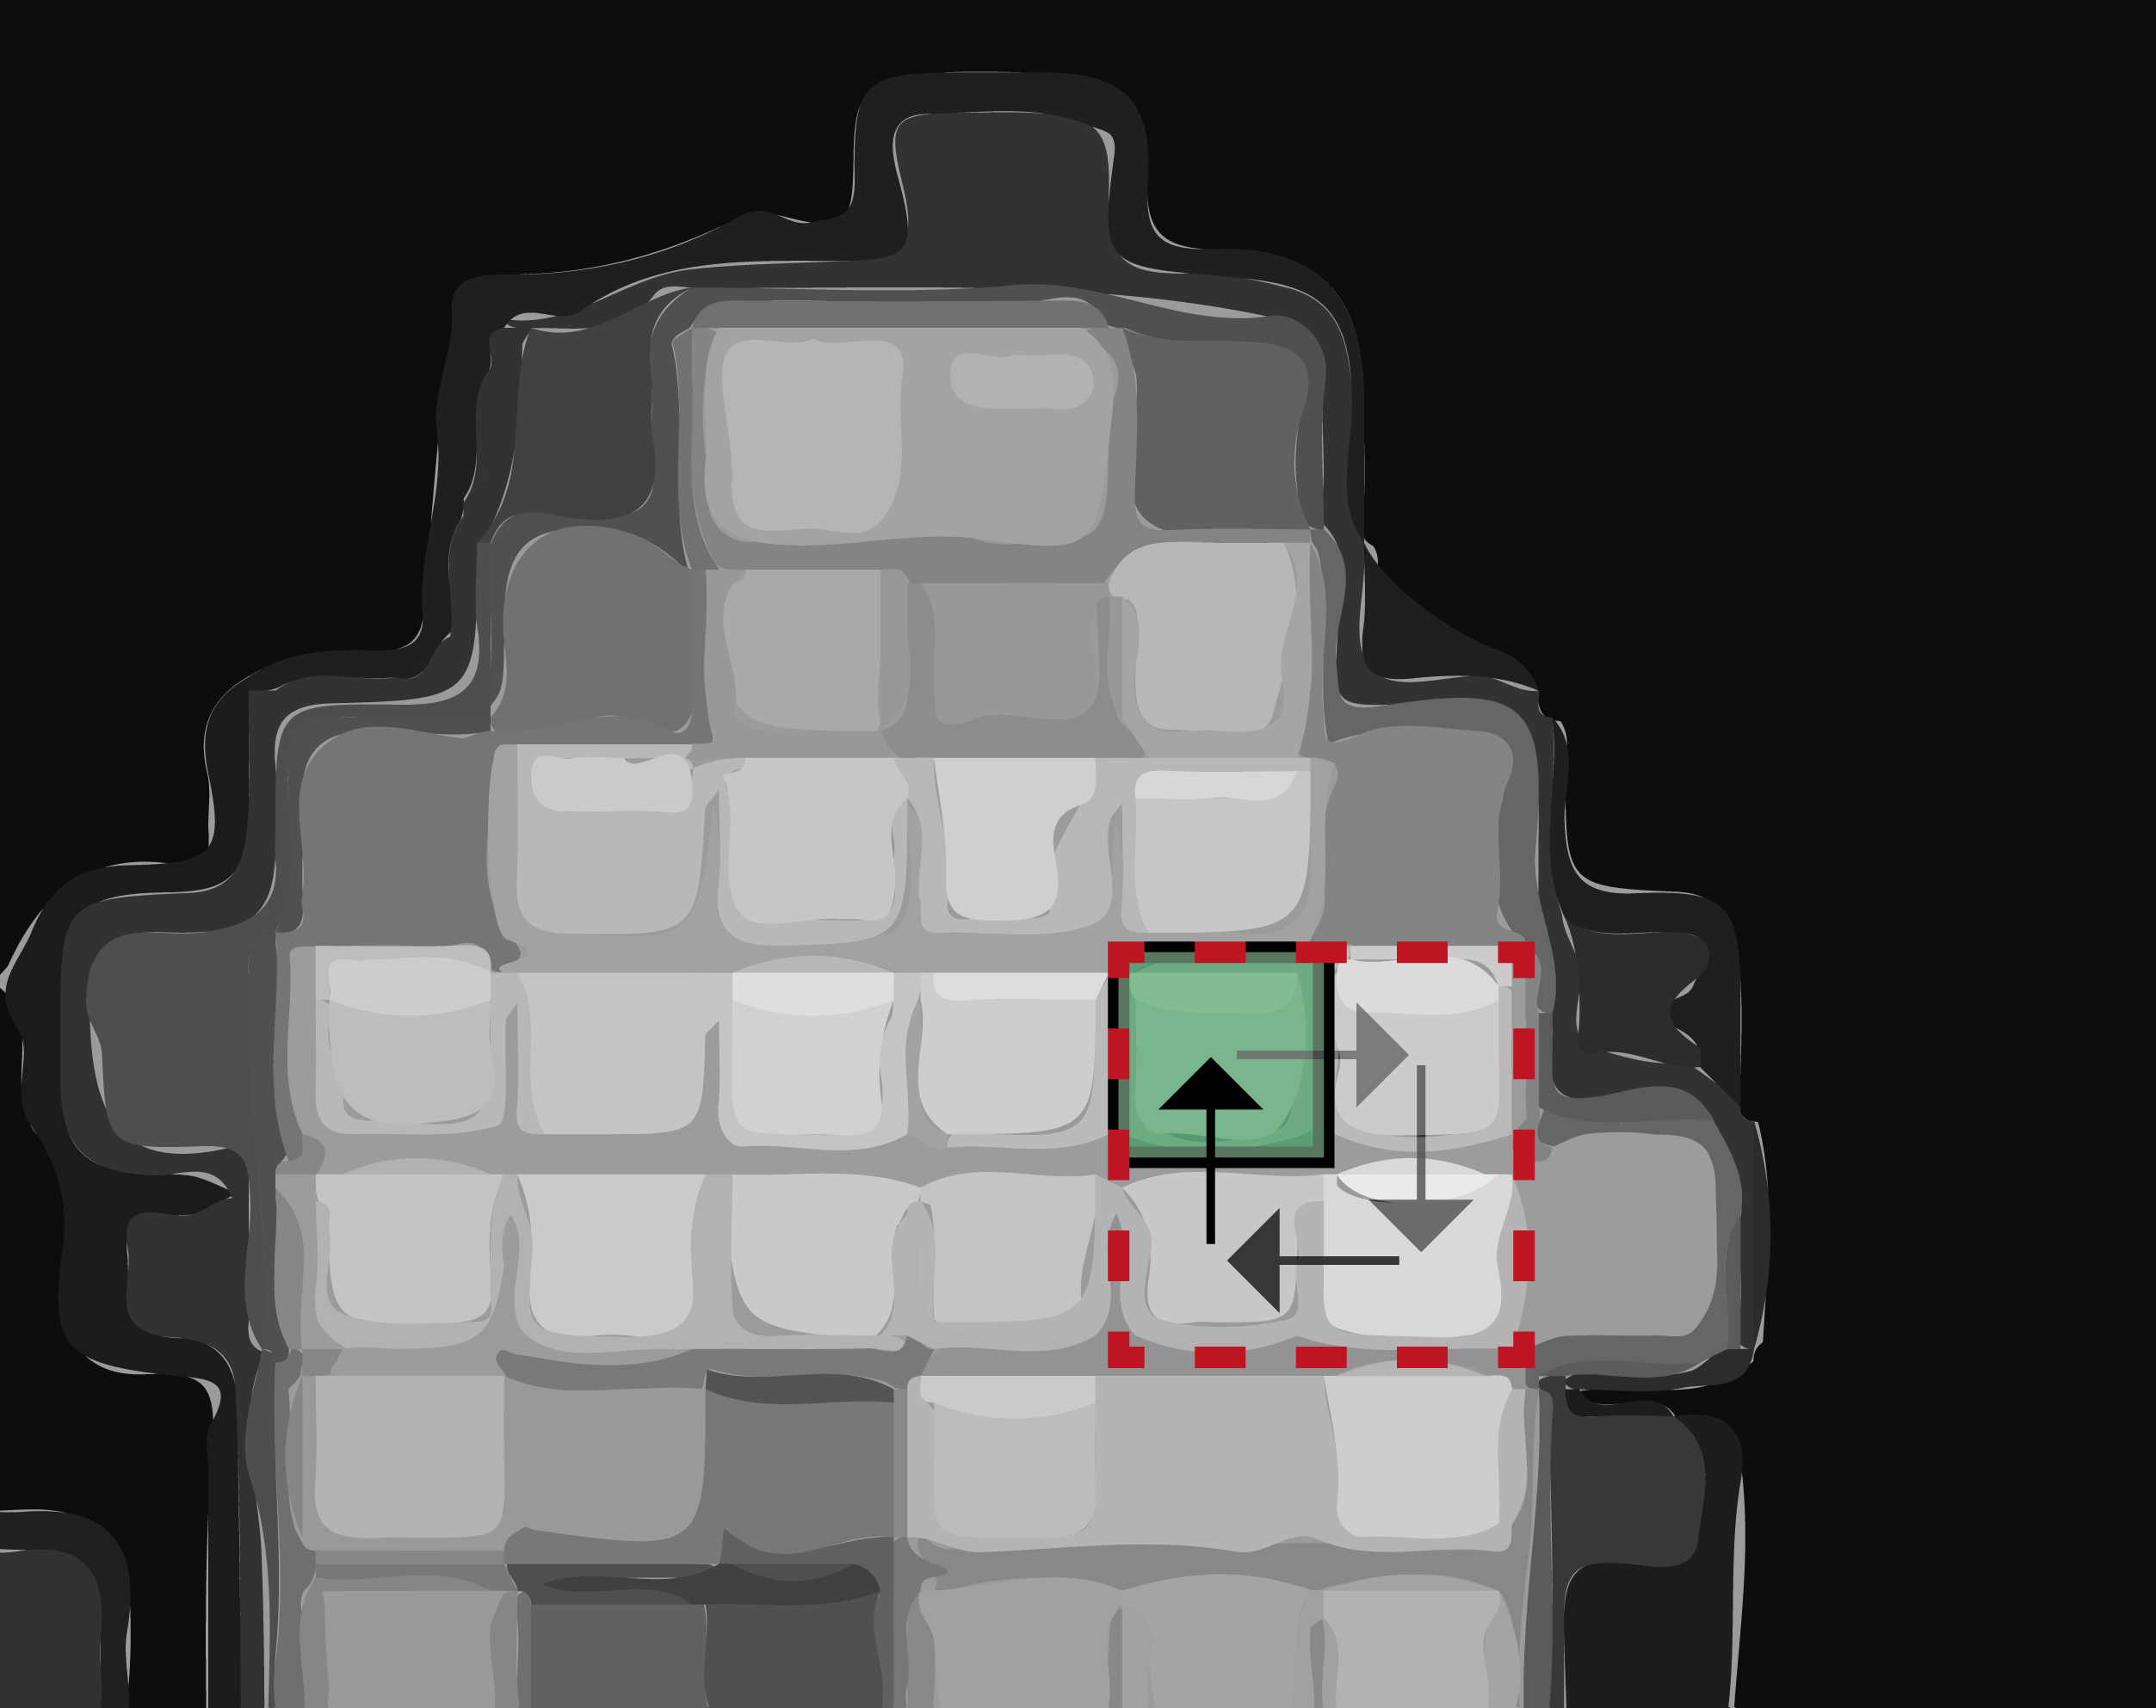
\includegraphics[width=0.75\textwidth]{PC2B_Meshing.jpg}
	\caption{PC2B Meshing Algorithm}
	\label{fig:pc2b_meshing}
\end{figure}

Each of the four vertices is converted back from the image plane to the cartesian coordinate system and contributes to build up the 3D surface. This process is repeated until every pixel of the image has been processed.

\subsection{Texture Coordinates and Normals}  \label{section_texture_coordinates_and_normals}

While the mesh is being generated, texture coordinates and normals are being calculated, too. Texture coordinates vary from 0.0 to 1.0 in the x and y direction, respectively. Real time computer graphics denote the texture coordinate axes as s and t, 3D software applications tend to name them u and v. By dividing the current pixel coordinate on the image plane by the width and height of the image, respectively, the coordinates can be normalized to get the texture coordinate. 3D Applications use the texture coordinate information to properly map an image texture (in our case the colormap) onto the 3D surface.


\begin{figure}[h]
	\centering
	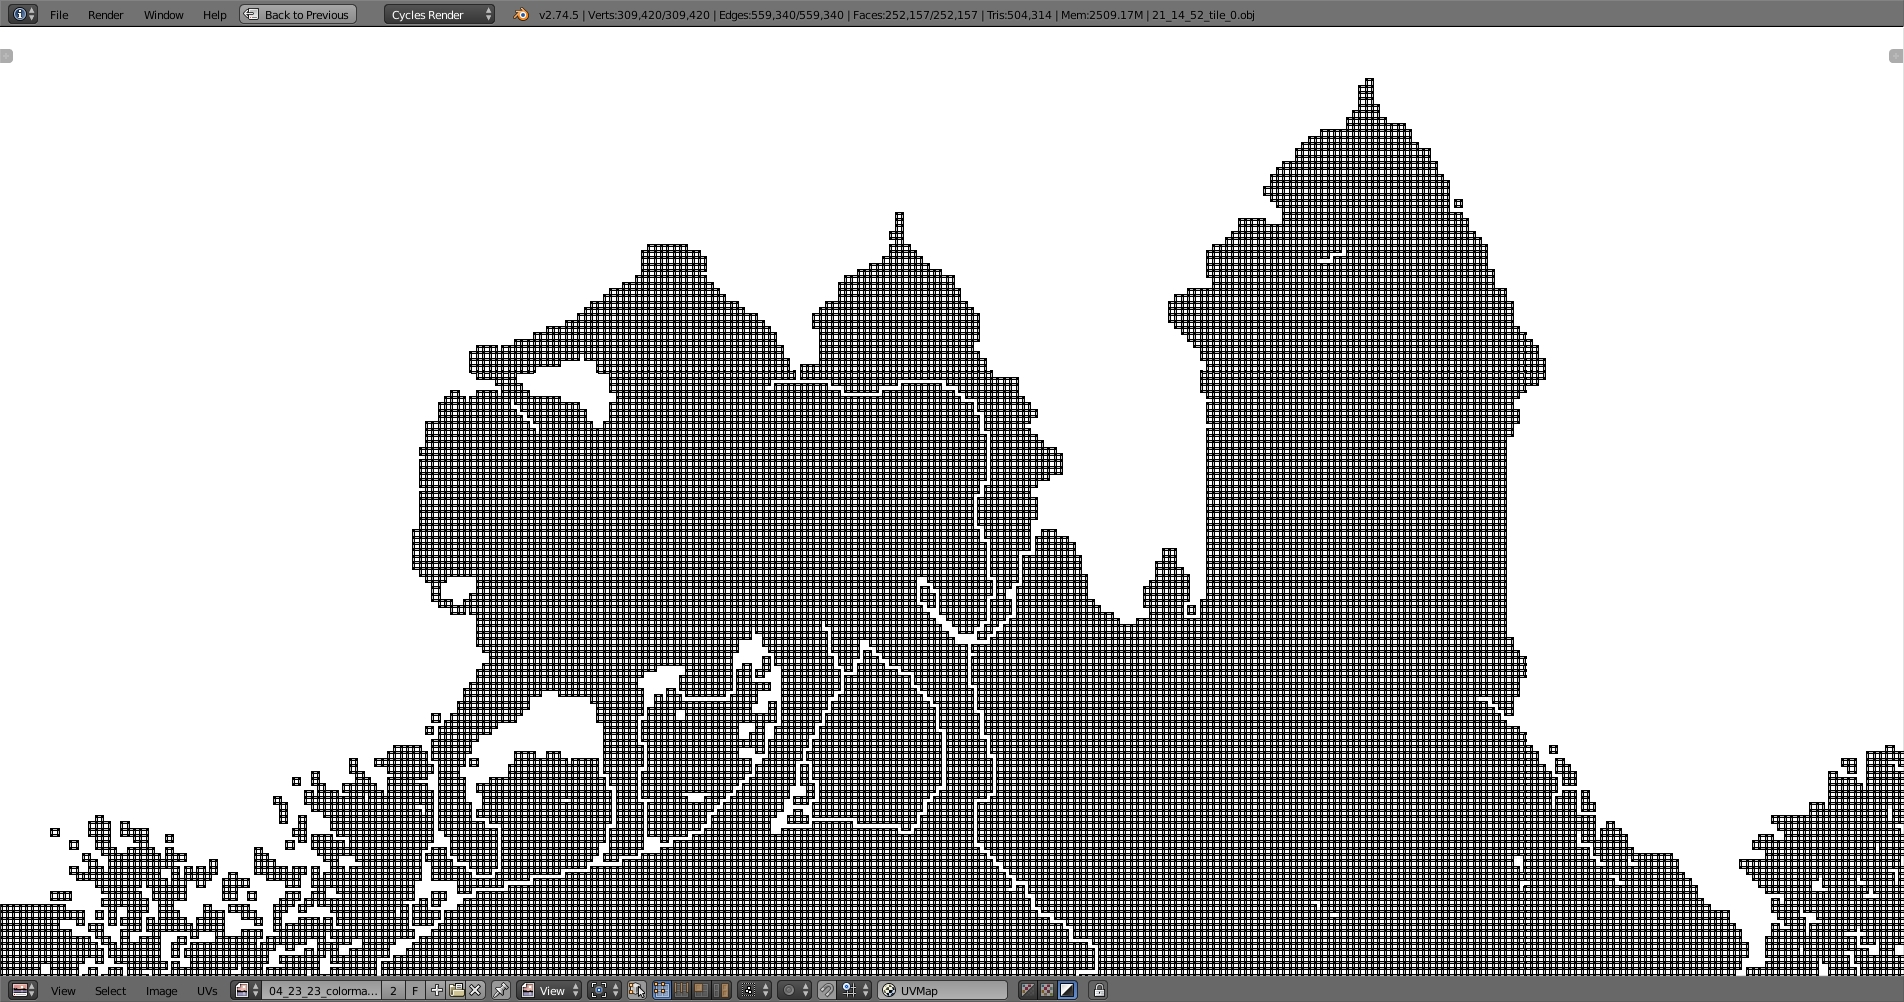
\includegraphics[width=1.0\textwidth]{PC2B_TextureCoordinates.jpg}
	\caption{PC2B Texture Coordinates viewed in Blender}
	\label{fig:pc2b_texture_coordinates}
\end{figure}


Calculating normals is accomplished by determining the cross product of the two vectors forming the current quad. It may happen that a polygon will get distorted at locations where the depth image values change quickly. Hence, the four-sided polygon is divided into two triangles and normals are generated for each of them. Normals are very useful to test certain properties of the mesh. This research uses normals to determine if a face is oriented perpendicular to the center of the panorama. Computing the dot product of a normal and a vector from the origin to the face returns the cosine of the angle between those two vectors. This is used in PC2B to discard polygons which would normally distort the mesh, as shown here:

\begin{figure}[h]
	\centering
	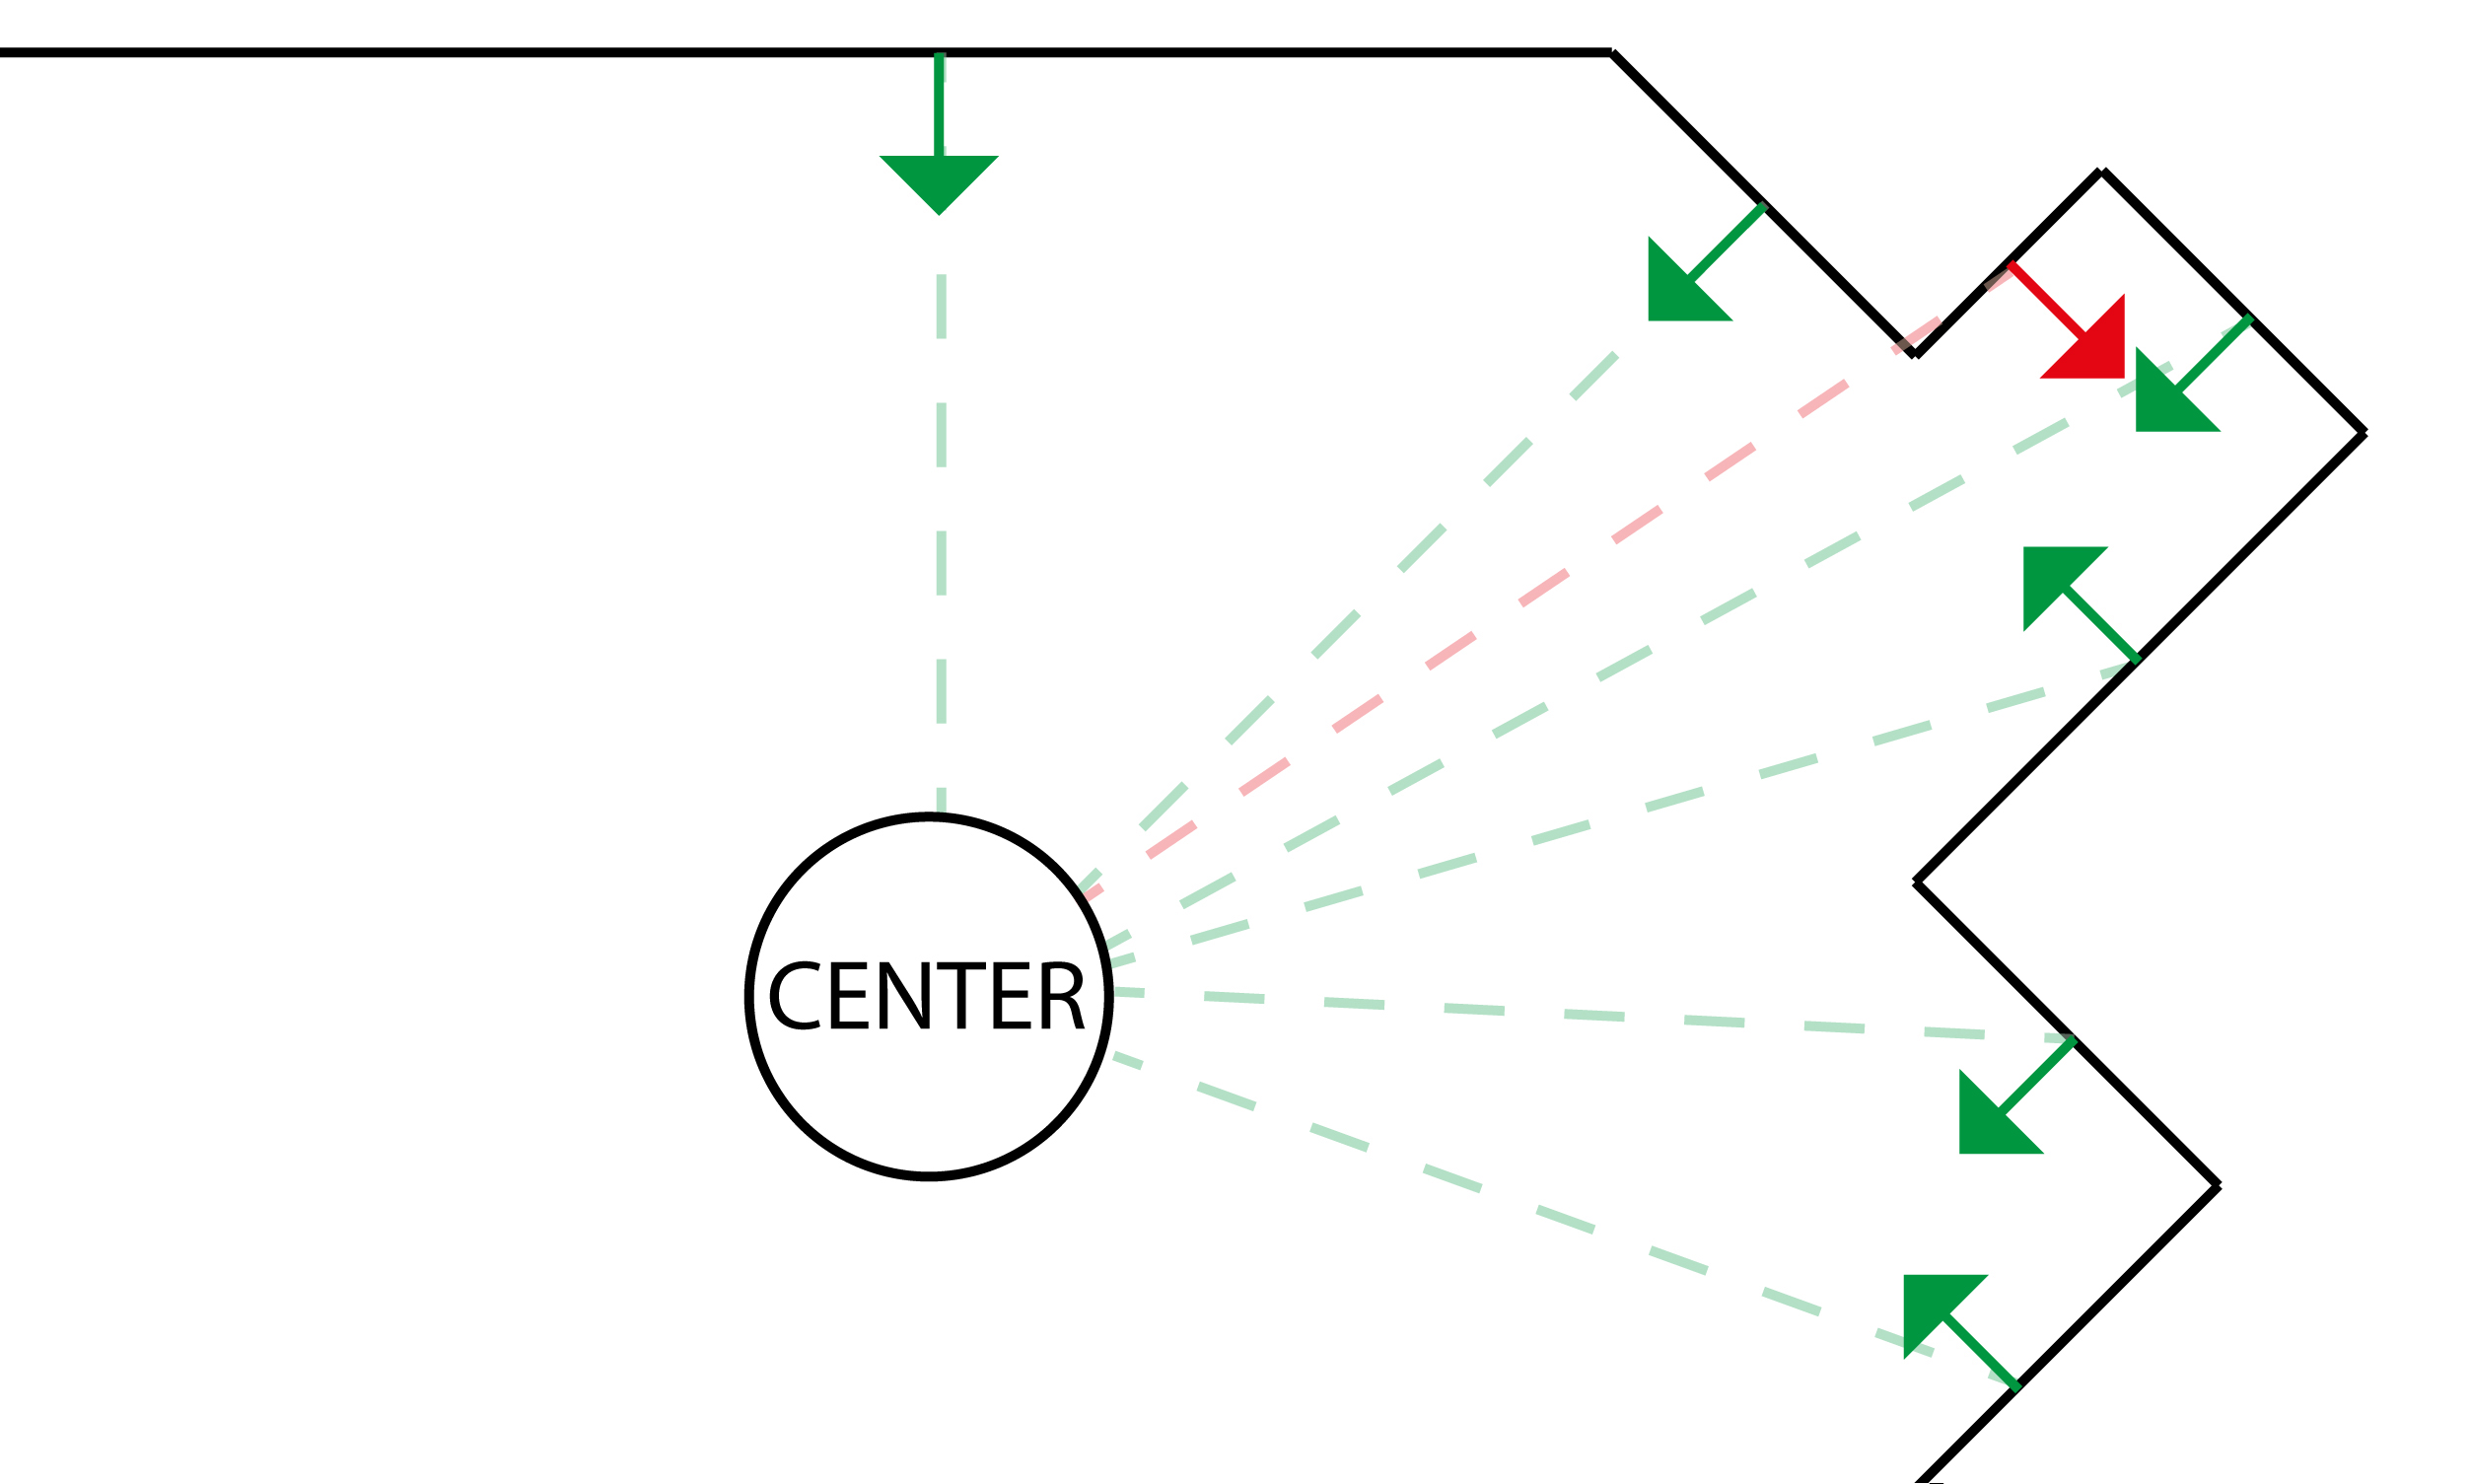
\includegraphics[width=0.75\textwidth]{PC2B_Normals.jpg}
	\caption{PC2B Normal filtering concept}
	\label{fig:pc2b_normals}
\end{figure}

This improvement cleaned up the generated mesh, since a lot of faces have been created in undesirable places.


\begin{figure}[h]
	\centering
	\begin{subfigure}[b]{0.45\textwidth}
		\centering
		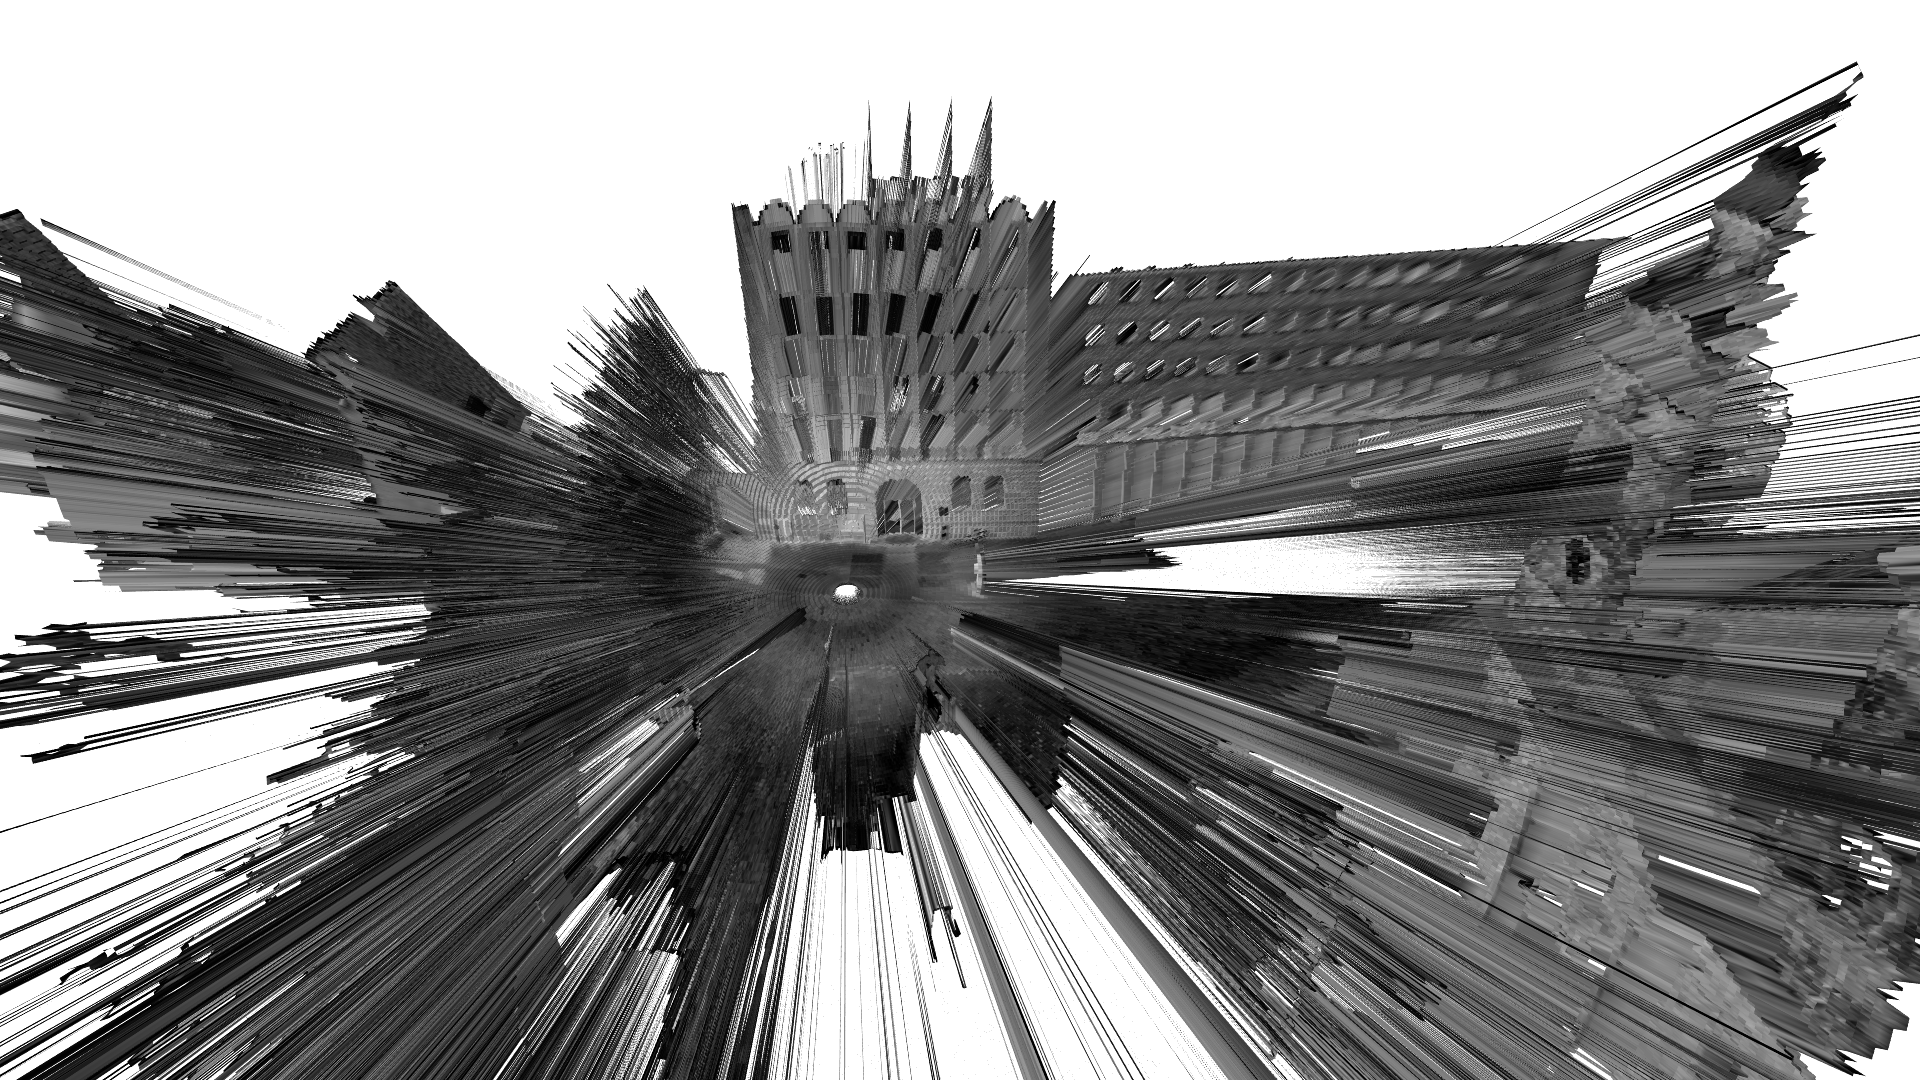
\includegraphics[width=\textwidth]{PC2B_Normals_off.png}
		\caption{Without normal filtering}
		\label{fig:PC2B_normals_off}
	\end{subfigure}
	\hfill
	\begin{subfigure}[b]{0.45\textwidth}
		\centering
		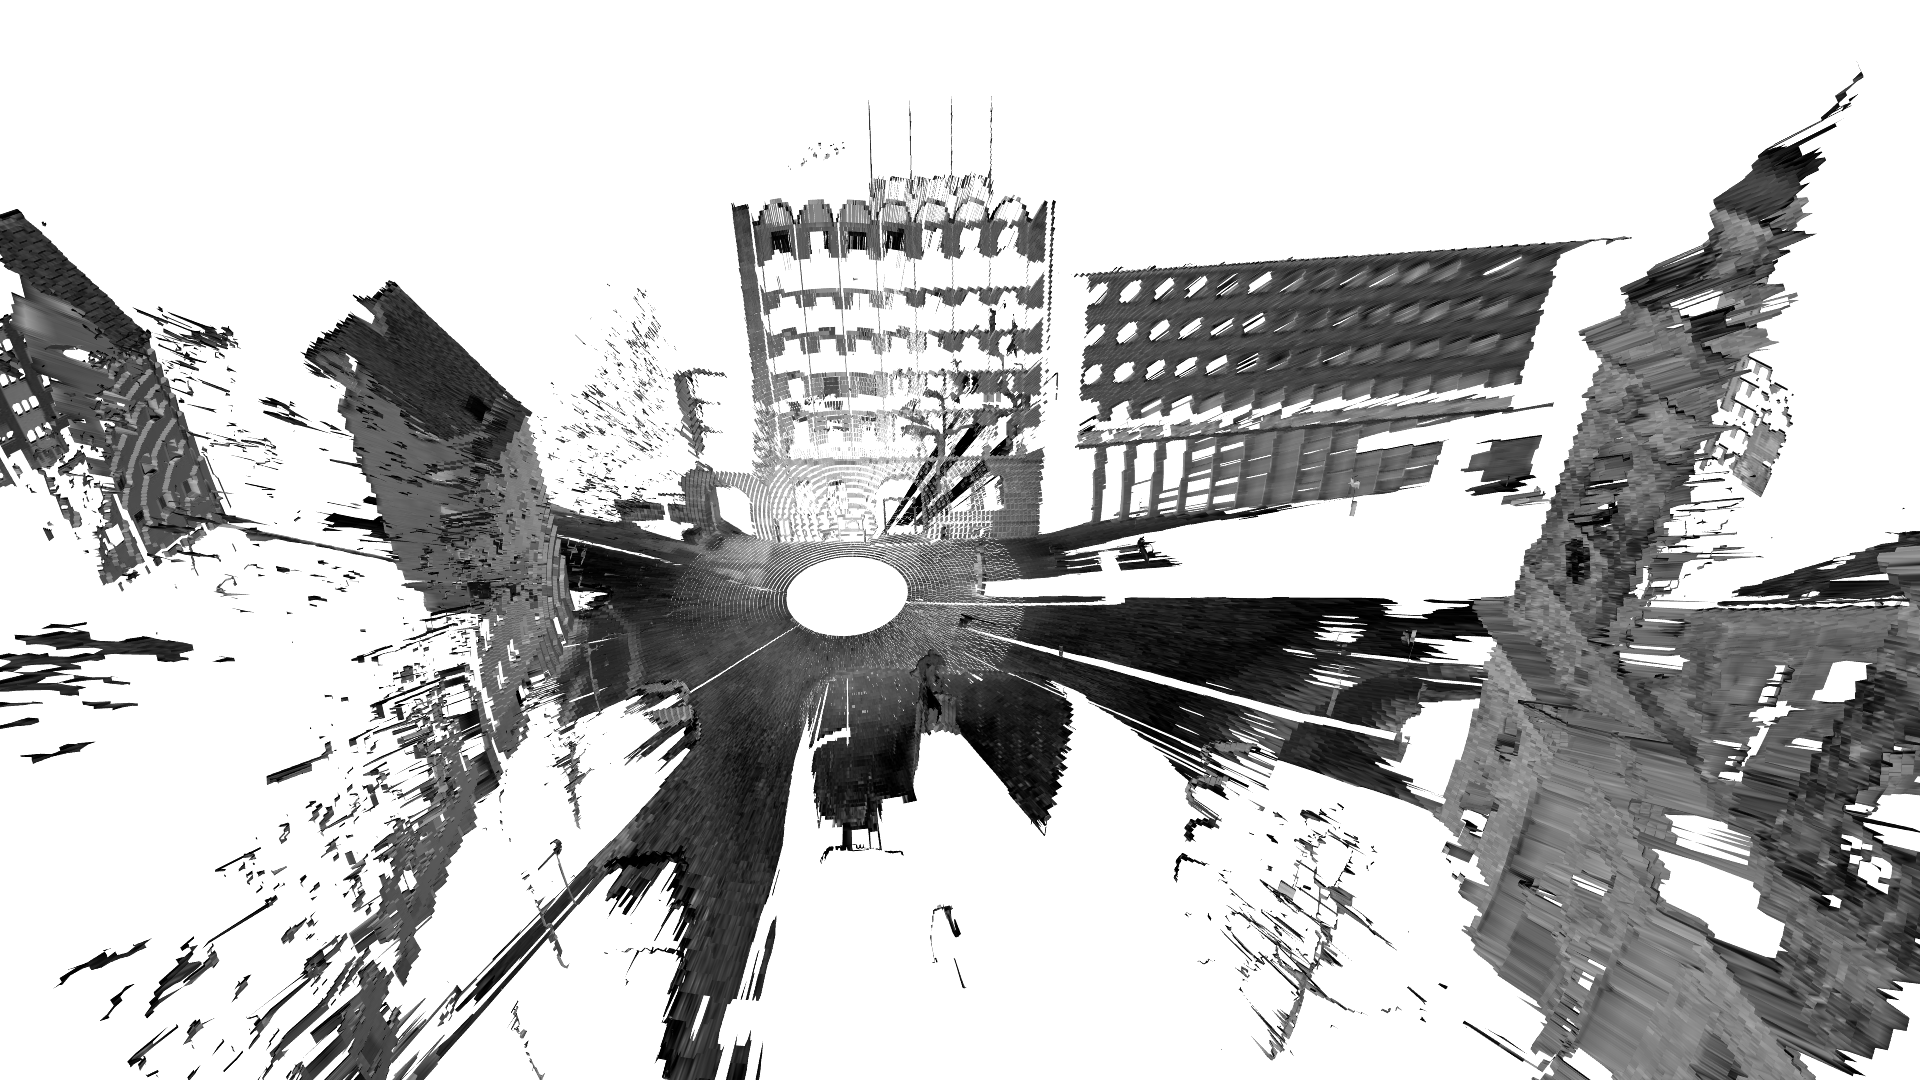
\includegraphics[width=\textwidth]{PC2B_Normals_on.png}
		\caption{With normal filtering}
		\label{fig:PC2B_normals_on}
	\end{subfigure}
	\caption{The generated mesh before and after normal filtering in PC2B}
	\label{fig:PC2B_normal_filtering}
\end{figure}


\subsection{OpenGL Point Cloud Viewer}

During the development of PC2B, it turned out that debugging would be easier if data is visualized simultaneously while importing and meshing. To that end we implemented a point cloud viewer. Initially it displays the coordinate axes. While importing it displays, at maximum, three million points from the point cloud file and during meshing it displays the final 3D panorama mesh.

\begin{figure}[h]
	\centering
	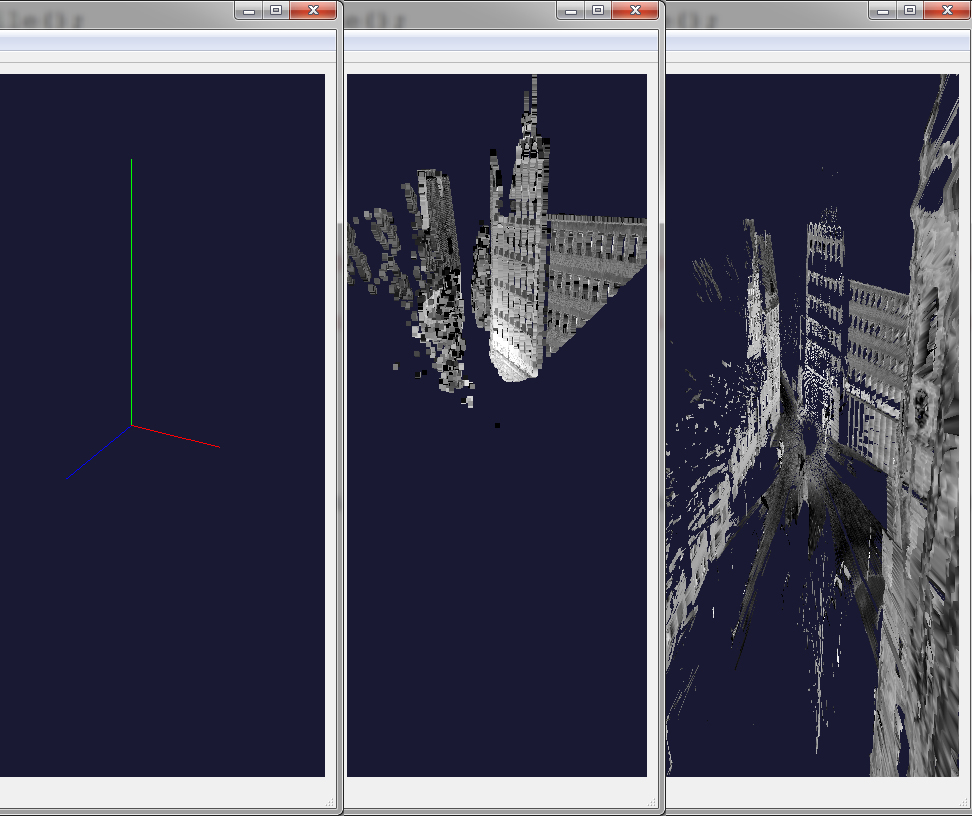
\includegraphics[width=0.5\textwidth]{PC2B_OpenGL_Viewer.jpg}
	\caption{PC2B OpenGL Viewer}
	\label{fig:pc2b_opengl_viewer}
\end{figure}

The Qt framework offers its own implementations to utilize OpenGL for drawing. Setting up the basic functionality within Qt was done with the help of a Russian video tutorial (see Enzhaev 2014 \parencite{ytQtOpenGL}). Using modern OpenGL drawing code was important to be able to handle millions of points and render high-resolution 3D meshes in real time.


\subsection{Mesh Exporter}

As a last step the generated mesh needs to be exported. Just like for importing, there is a huge amount of file formats available to export to. One format had to be chosen that supported at least vertices, texture coordinates and faces.

\subsubsection{.obj}

The .obj format is one of the most popular, and possibly easiest to understand, file formats to save 3D geometry with not only vertices, but normals, texture coordinates, parametric surfaces, splines and much more. With .obj files, usually .mtl files are saved. Those Material Template Library files store additional information about the 3D material, such as ambient, diffuse or specular color, transparency and reflection settings, or filepaths to image textures. It was the first choice when testing the mesh export from the converter software and examining it in Blender. Furthermore this file format can be used with almost any other 3D software application.

\subsubsection{.blend}

A personal goal for this research was to implement a .blend export feature to allow for a native importing of the panorama mesh into Blender. However, this goal was not reached in this project. As it turned out, exporting the binary Blender file format was quite complicated, due to its versatile structure. An experienced Blender Developer, Jeroen Bakker, stated in 2009: “[...] When implementing loading and saving blend-files in a custom tool the difficulty is the opposite. In a custom tool loading a blend-file is easy, and saving a blend-file is difficult. [...]” (see Bakker 2009 \parencite{webMysteryOfTheBlend}). At least, implementing the feature with the limited time for the thesis was not feasable.

\subsubsection{custom format}

Even the Blender community suggested to not use the .blend format directly, but rather try a custom binary format (see thread on BlenderArtists \parencite{webBlenderArtistsBlendExport} by the author). Implementing such a binary file format would result in a fast and memory efficient way to exchange the mesh between PC2B and Blender as well as a comfortable solution for users, since the file could automatically be openend with Blender after meshing is finished. In this research the custom file format was omitted in favor of the aforementioned .obj file format. However, it is under consideration to be implemented eventually.

\subsection{Optimizations}
\label{section_optimizations}

The initial algorithms and approaches had some flaws, which needed to be eliminated to achieve a clean mesh out of the converter. Further, there are still some issues with the converter software which we would like to address briefly:

\subsubsection{Various import settings}

The point cloud file which is going to be meshed could need some minor adjustments, such as a predefined translation along a 3D vector, or it might have a different orientation. In addition, the maximum scan distance or the normal angle threshold for discarding normals (see Section \ref{section_texture_coordinates_and_normals}) could need tweaking. Those settings are exposed to the user in PC2B.

\subsubsection{Panorama pixel depth testing}

It might happen that two or more points from the point cloud fall into the same pixel in the 2D panorama. On the one hand this might result in a noisy image. On the other hand, this affects the generated mesh, if not handled with care. To avoid any errors, it is important to take only the closest point to the camera, instead of just letting every 3D point override the corresponding pixel in the image. This is implemented in the converter software.

\subsubsection{Panorama flipped horizontally}

The panorama images are currently flipped horizontally. This is not a serious issue, since the texture coordinates are created based on these images and therefore the texture is eventually applied correctly. However, this might be something to consider changing.

\subsubsection{Panorama noise reduction}

Since there is only a limited number of points, the panorama texture can get quite noisy or gaps can occur, especially with a higher resolution option set in the converter. A distinct change from light to dark gray values in the depth map will result in a noisy 3D surface as well.
To solve this issue, the image pixels could either be formed by averaging the values in a certain region or blurred by a user-defined amount.

\subsubsection{Remove doubles}

The meshing algorithm currently produces a very high point count in the .obj file. For Example: A quadruple resolution panorama with 2,198,528 vertices will be automatically decimated by 2,100,716 vertices using the "remove doubles" option in Blender 3D.
This could be solved by buffering the vertex data and using several passes for writing vertices, texture coordinates, and normals in the mesher algorithm. Every vertex would only be saved once and get referenced by its index when defining the individual faces.

\subsubsection{Tiling}

Due to the higher-resolution meshes being several megabytes in size and taking some time to import in Blender, this could also be optimized.
Depending on the resolution set by the user, the converter could create tiles. If, for example, a quadruple resolution is set, four tiles get created (that is four separate .obj, .mtl and image files). Another idea might be to provide users a tool to define custom borders in the panorama to only export specific parts of the scan.

\subsubsection{Quantized 3D surface}

The panoramic image pixels are stored as 8-bit unsigned integer values at the moment. This does not allow depths in very fine steps, as 8 bit can only store $2^{8}$ = 256 values. A good solution would be to store the values with at least floating point precision. This would also eliminate the need for the user to specify a maximum scan resolution. Most importantly the mesh quality would be greatly improved, which we believe would be highly appreciated by artists.

\subsubsection{Better memory management}

Almost all of the aforementioned issues have one reason in common: they require quite a lot of memory, and thus better memory management in order to be resolved. PC2B cannot be run on older systems with 1 GB RAM at the moment, because of the allocation of a fixed memory block for the OpenGL point cloud viewer. A better approach would be a dynamic memory allocation. In this regard the use of the C++11 standard with smart pointers might lead to significant improvements.

Although PC2B works well without those optimizations, they would greatly benefit the output of the converter software, in our view.